\documentclass{article}
\PassOptionsToPackage{numbers}{natbib}
\usepackage[education, final]{neurips_2026}
\usepackage[utf8]{inputenc}
\usepackage[T1]{fontenc}
\usepackage{hyperref}
\usepackage{booktabs}
\usepackage{microtype}
\usepackage{graphicx}
\hypersetup{colorlinks=true, urlcolor=blue, linkcolor=blue, citecolor=blue}
\setlength{\parskip}{3pt}
\setlength{\parindent}{0pt}
\newcommand{\blk}[1]{\vspace{1pt}\noindent\textbf{\normalsize #1}\hspace{0.5em}}

\title{Test-Time Compute Allocation: Search vs.\ Verify}
\author{Author Name \\ Affiliation}

\begin{document}
\maketitle

\blk{The Concept}
This page is the course's entry point: it defines the concept below, states the learning objectives, links the frontier papers, and routes you to the video, slides, and notebooks.

The concept taught in this course is test-time compute allocation: given a fixed inference budget (a fixed number of model calls), how should a model divide it between search and verification? Search generates many candidate answers and aggregates them, for example by majority voting. Verification generates fewer answers and checks each one with a judge (a verifier). Search carries a mathematical guarantee: with independent candidates and accuracy p above 1/2, the failure probability of majority voting falls exponentially in N; verification has no such guarantee, and only helps when the judge can tell good answers from bad ones. In this course the judge is the model grading its own answers; our measurements show it is weak, barely separating correct from incorrect candidates. Under a weak judge and a moderate budget (the setting of this course), search usually wins; the best split depends on your model, your judge, and your budget. Our measured setting (100 MATH 500 problems, 50 calls per problem, Qwen3-4B, three seeds) is in Table~\ref{tab:worked}.

\begin{table}[h!]
  \caption{Measured accuracy on the 100-problem MATH 500 subset (Qwen3-4B, three seeds, budget 50 calls per problem).}
  \label{tab:worked}
  \centering
  \small
  \setlength{\tabcolsep}{3pt}
  \begin{tabular}{llcc}
    \toprule
    Strategy & Split & Accuracy [95\% CI] & Reference \\
    \midrule
    Search & 50 candidates, majority vote & 0.853 [0.81, 0.89] & \citep{iclr2025scaling} (Majority) \\
    Search + light verification & 25 candidates $\times$ 1 check & 0.717 [0.67, 0.77] & -- \\
    Verification & 5 candidates $\times$ 9 checks & 0.753 [0.70, 0.80] & \citep{iclr2025scaling} (PRM weighted) \\
    \bottomrule
  \end{tabular}
\end{table}

\blk{Leveling and Prerequisite Knowledge}
Level 1 (no prerequisites): watch the five-minute video and read this page; you get the core trade-off in plain terms. Level 2 (systematic): work through the notebooks and slides; this path is aimed at graduate students and early-career researchers in LLM reasoning and is adaptable for advanced undergraduates. Before starting, you should answer: (1) Why does an LLM reload all weights for every token? (2) If each candidate is right 30\% of the time, what is the chance that majority voting over three independent candidates is right? (3) What do MATH and GSM8K measure, and how do their difficulties differ? Answers are built into Notebook 00.

\blk{Learning Objectives}
By the end of this material, learners will be able to: \textbf{Level 1}: explain the search--verification trade-off in plain language, naming the two conditions under which search wins (a weak judge, a moderate budget); evidence: a 30-second retelling. \textbf{Level 2}: (1) estimate a model's failure rate with a simplified majority-voting model and predict the candidate count N needed; evidence: a calculation. (2) plot their own budget--accuracy curve with at least two data points and read the six-model curve family; evidence: a plot plus a written reading. (3) given a new task and a fixed budget, reason out the best search--verify split from the model's accuracy and the judge's strength; evidence: an analysis report. (4) advanced: judge whether a research paper's baselines are fair; evidence: a critical report.

\blk{Linked Papers}
Test-time compute allocation is in active use at the frontier; each paper below builds on it. \emph{Scaling LLM Test-Time Compute Optimally} \citep{iclr2025scaling} studies the allocation problem directly: compute-optimal splits beat fixed best-of-N by up to 4$\times$, and with a strong judge (e.g., a trained reward model), verification-guided search wins at low to moderate budgets. \emph{Sample, Scrutinize and Scale} \citep{icml2025sample} pushes the allocation toward verification at very large budgets, where sampling-based search with self-verification keeps scaling. \emph{Let Me Think!} \citep{neurips2025letme} allocates the budget between one long chain and many short ones, showing serial expansion can be exponentially better. \emph{Provable Scaling Laws} \citep{neurips2025provable} gives pairwise-comparison aggregation (a search-style strategy) a guarantee even below $p = 1/2$. \emph{When to Solve, When to Verify} \citep{colm2025whento} asks the same allocation question with a generative reward model, finding self-consistency (search) more compute-efficient than verification for most budgets, which is exactly the weak-judge regime that this course measures.

\blk{Teaching Materials Summary}
All materials are original and were created for the NeurIPS 2026 Education Track; everything lives in \url{https://github.com/Solitus0726/search-vs-verify-course}. Suggested order: start with the self-check (Notebook 00) to find your path, then follow its materials in the order shown in Figure~\ref{fig:learning}, with the slides as a reference for the math. The learning path in Figure~\ref{fig:learning} routes you through these materials. The video (about five minutes) explains the trade-off in plain terms. Notebook 00 runs the three-question self-check, and failing any question routes you to the supplementary materials. Notebook 01 plots budget--accuracy curves and reads the six-model family (p from 0.37 to 0.73); Notebook 02 finds the optimal split under the budget identity $N\times(1+M)=50$; Notebook 03 predicts the best split for GSM8K and tests it; Notebook 04 is the report template. The slides and strategy diagram add the formal math and a one-page visual summary. The scripts and data make every result reproducible: about one to two hours from scratch, or instantly with the pre-computed cache included in the repository.

\begin{figure}[h!]
\centering
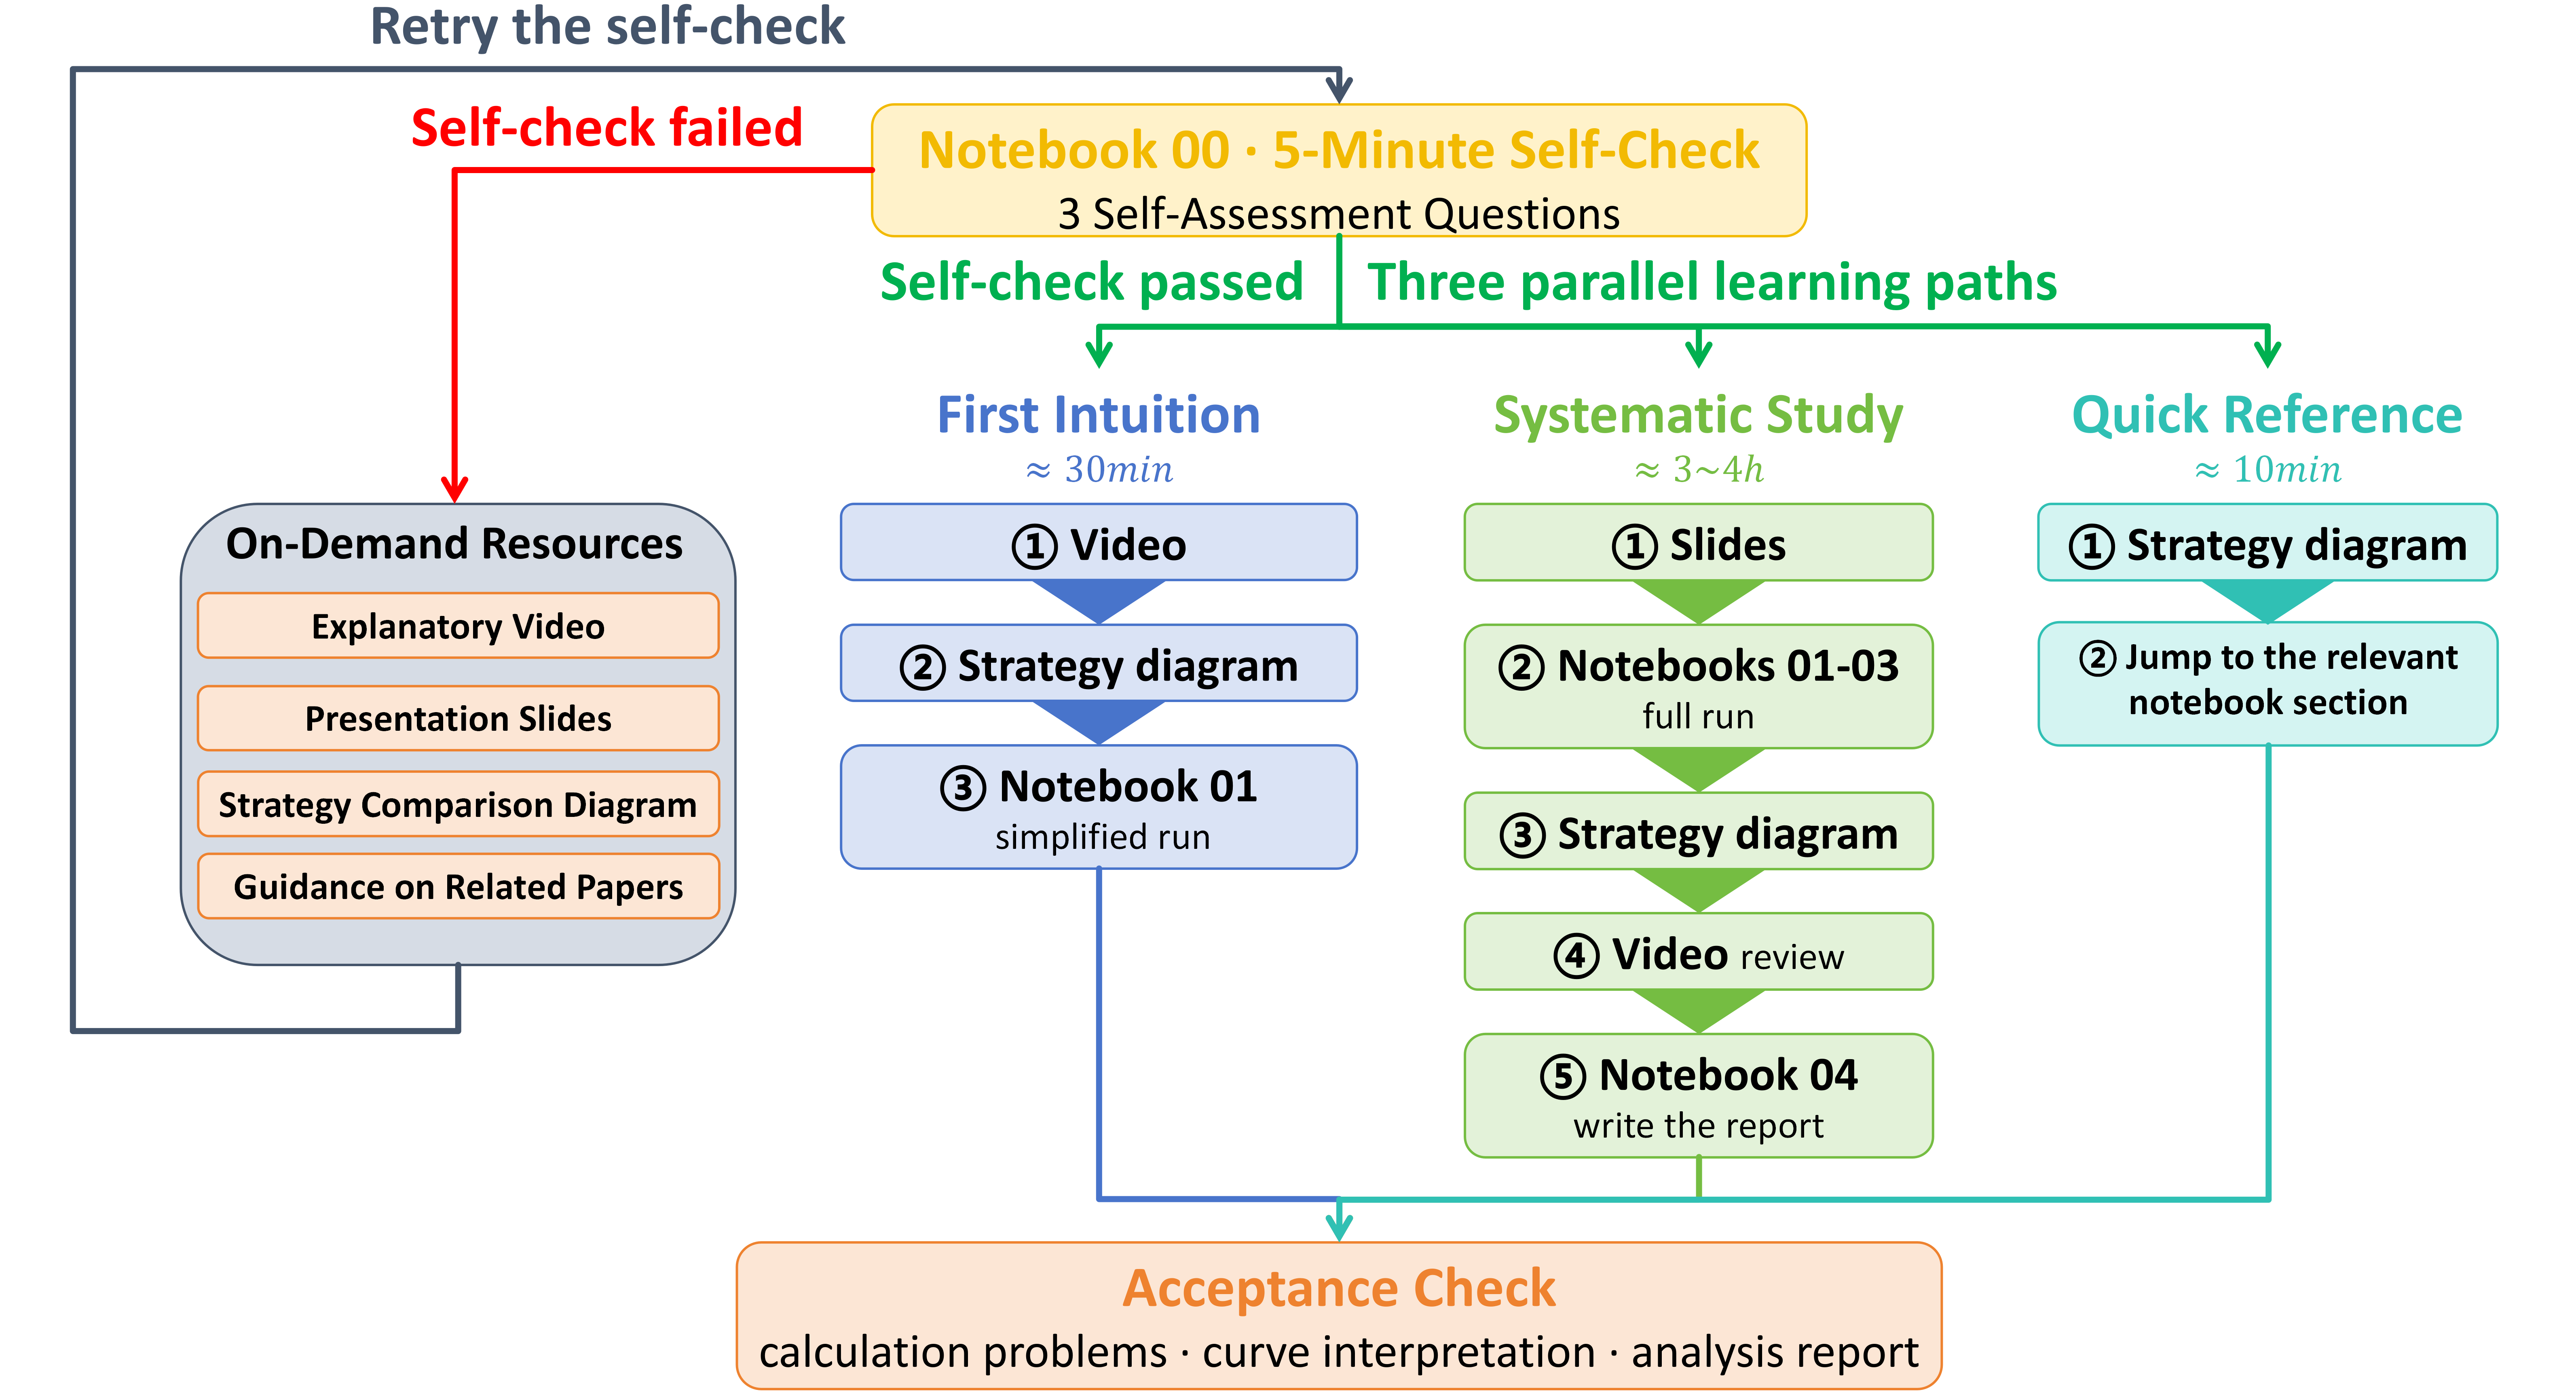
\includegraphics[width=\textwidth]{learning_path.png}
\caption{Learning path: a five-minute self-check routes you to supplementary materials or to one of three material sequences (intuition-first, systematic, quick reference), ending at the acceptance checks.}
\label{fig:learning}
\end{figure}

\bibliographystyle{plainnat}
\footnotesize
\bibliography{refs}

\end{document}
